\section{Related Work}
\textcite{andreasen2017survey} survey automated test generation in section 8 of their work\parencite[23-25]{andreasen2017survey}. They survey a total of 14 papers in this category and separate them into one of three approaches - explorations of the event space (concerning the order of execution of event handlers), explorations of the value space (choice of values for inputs), and generation of assertions \parencite{andreasen2017survey}. 
In the event space category their findings include 
approaches based on random executing of event handlers, heuristic methods, based on observations of read and written values in order to exclude handlers with no interaction, and a tool for measuring the performance impact of handlers. Most of their findings in the value category focus on concolic execution \parencite{godefroid2005dart}, a technique for generating concrete inputs (test cases) in order to maximize test coverage. Almost all of their finding in the assertion generation category are based on
Crawljax \parencite{crawljax2021Feb}, an event-driven open source web crawler for dynamic Ajax-based Web applications, which is also capable of exploring JavaScript-based \gls{dom} state changes.
A table with a more detailed overview can be found in \parencite[24]{andreasen2017survey}.

Model checking of Web applications - a method for checking whether a finite-state model of a system conforms to a specification, is explored in \parencite{zhang2019scenario} and \parencite{gao2019model}
\section{Scenario Testing of AngularJS-based Single Page Web Applications}
\textcite{zhang2019scenario} present a method with the goal of achieving better understanding of AngularJS-based \glspl{spa} and also devise a way to specify test coverage criteria based on it. At the center of the proposed method are Interaction Diagrams, which are used to model the overall data and control flow of an application.\parencite{zhang2019scenario}

\subsection{Abstract Syntax}
\textcite{zhang2019scenario} model an AngularJS-based \gls{spa} as a tuple ($T$, $C$, $D$, $E$), where

\begin{itemize}
  \item $T$ is a HTML template, consisting of a set of HTML tags (widgets) ($T = \{h\}$)
  \item 
  $C$ is a controller (view-model), written in JavaScript. It is modeled as a tuple ($V$, $F$, $\$scope$), where $F$ and $V$ are top level variables and functions, respectively, and $\$scope \in V$ is a distinguished element of $V$. Further $V(\$scope)$ and $F(\$scope)$ denote all variables and functions of $\$scope$ ,respectively. $W = V \setminus \{\$scope\}$ denotes top level variables not in scope. Additionally $init \in F$ is defined as an initialization function.
  \item $D$ is a set of \glspl{databinding} between HTML tags and variable properties of $\$scope$ $ D \subseteq \{(h,V(\$scope) \cup F(\$scope))\}$. Given $d = (n,o)$ $source(d) = n$ and $target(d) = o$. For two-way bindings $D' \subseteq D$ and $\forall d \in D'$ $target(d) \in V(\$scope)$.
  \item $E$ is a set of event handler bindings between HTML tags and function properties of $\$scope$: $E \subset \{(h,F(\$scope))\}$. In addition, for each function $f \in F \cup F(\$scope)$, $R(f) \subseteq V \cup V(\$scope)$ and $W(f) \subseteq V \cup V(\$scope)$ are defined as the values that the given function reads from and writes to. $Inv(f) \in F $ are defined as the functions invoked by $f$. \parencite{zhang2019scenario}
\end{itemize}
\subsection{Interaction Diagrams}
\label{intro:zhang_interaction_diagrams}
\textcite{zhang2019scenario} define interaction diagrams as a directed graph ($N$, $E$). 

\subsubsection{Nodes}
The set of nodes $N$ is defined as the union of $N_H$ (HTML tag nodes), $N_{\$scope}$ (databindings and events) and  $N_{js}$ (JavaScript functions). 

Formally $N_H = \{n_h | (h,v) \in D\}$ , $N_{\$scope} = \{n_v | (h,v) \in D\} \cup \{n_e | (h,e) \in E\}$ 
$N_{js} = \{n_v | v \in W\} \cup \{n_f | f \in F\} $ The initialization node, $n_{init}$, is distinguished by an incoming arrow without a starting vertex.

\subsubsection{Edges}
The set of edges $E$ is a combination of seven sets:

\begin{itemize}
  \item \glspl{databinding} are defined as $e_d = (target(d),source(d))$ , $E_{data} = \{e_d |  d \in D \}$. Additionally for two-way bindings: if $d \in D'$ also create $e'_t = (source(t),target(t))$ and $E'_{data} = \{e_d |  d \in D' \}$
\item Events are defined as ($E_{event}$) $(h,f) \in E$
\item Variables methods write to - $E_{W}$, $(f,v)$ where $f \in F \cup F(\$scope), v \in W(f)$
\item Variables methods read from - $E_{R}$ $(v,f)$ where $f \in F \cup F(\$scope), v \in R(f)$
\item Methods, invoked by other methods - $E_{Inv}$ $(f,v)$ where $f \in F \cup F(\$scope), v \in I(f)$
\item  default values of widget set by the \textit{init} function
$E_{init}$ default values of widgets 
for each $h \in T $ where $ \nexists v | (h,v) \in D$ create an edge $(h,v)$ 
\end{itemize}
\textcite[9]{zhang2019scenario} provide a more detailed explanation of the above, including examples.
 

\subsection{Testing and Interactions}
\textcite{zhang2019scenario} define an \textit{interaction} as a round of user input including updates to the widgets by the application. Interaction can be triggered explicitly by the user (by invoking an event handler) or implicitly while the user is updating data \parencite{zhang2019scenario}.

Given Interaction Diagrams as described in \ref{intro:zhang_interaction_diagrams}, it is possible to derive which widgets get updated by a user input action or setup by the initial function. \textcite{zhang2019scenario} define it formally as follows:
\begin{quote}
\label{quote:interactions}
Given a node $n \in N_H \cup \{init\}$, we say a node $m \in N_H$ \textit{reacts} to $n$ iff
  \begin{enumerate}
      \item $\exists n_0,n_1,n_2, \ldots,n_k \in N, n_0=n,n_k=m$ such that for each $0 \leq i < k  $ $(n_i,n_{i+1}) \in E$, and 
      \item $\forall n_p, 1 < p \leq k$ and $\forall e \in E, target(e)= n_p$ it holds that $e \notin E_{event}$  
  \end{enumerate}
  We write $l(n)$ for the set of all nodes representing the widgets that react to $n$. This set contains the widgets that are automatically updated upon user input,
  and thus constitute an interaction.
  \end{quote}

For example, in order for the widget $n$, which was clicked by the user, to update the widget $m$, $m$ must be reachable from $n$ by following the directed edges of the interaction diagram and only the first edge can be an event-handling edge.

What is crucial is that the interactions $l(n)$ define an upper bound of what can be updated, i.e. what \textit{might} get updated. Nevertheless, this information is sufficient in order to be able to define coverage criteria \parencite{zhang2019scenario}.

\subsection{Coverage Criteria}
Interactions should not be tested in isolation and in order for tests to make sense, interactions as preconditions are required \parencite{zhang2019scenario}. 
In order to define coverage criteria, \textcite{zhang2019scenario} extend their notation, as described in \ref{intro:zhang_interaction_diagrams}, by defining $\mathcal{I}  = \{w\in T | l(w) \neq \emptyset \}$ all widgets, that interactions.

A sequence of user interactions, including the initial function is referred to as a \textit{scenario} $A=(a_0,a_1,\ldots, a_n)$ where $a_0=init$ and $\forall0 < k \leq n, a_k \in \mathcal{I}$. The widgets, to which a scenario reacts, are equal to the widgets to which the last widget in the scenario reacted to - $l(A)=l(a_n)$. 


The set of scenarios is generated by starting with the initial scenario, containing only the initial function $S_0 = \{(init)\}$ and prolonged  iteratively by each widget, where the user can take an action. This is terminated once all $i \in \mathcal{I}$ are included in at least one scenario. 
Formally, define $A \oplus x = a_0,a_1,\ldots,a_n,x$ For $n > 0, S_{n+1}= \{ p \oplus x |p \in S_n, x \in l(p) \cap \mathcal{I}\}$ 

Based on the scenario sets \textcite{zhang2019scenario} define the following coverage criteria:
\begin{quote}
\begin{itemize}
  \item Each set $S_n$ of test scenarios should be tested.
  \item For each given $S_n$, each $p \in S_n$ should be tested.
  \item For each given $p$, each $w \in l(p)$ should be tested. That is, there should be a
  test case for each widget that may be modified after the scenario $p$.
\end{itemize} 
\end{quote}

\section{Scenario Testing}
Scenario testing, was originally introduced in \textcite{kaner2003power} and later as \textcite{kaner2013introduction}. The author defines scenarios as hypothetical stories, which aid a person in understanding a complex system or problem. Scenario tests are tests, which are based on such scenarios.  \parencite[1]{kaner2013introduction}
Further, \parencite[2-5]{kaner2003power} defines five characteristics, which make up a good scenario test -
A Scenario test must be
\begin{itemize}
     \item based on a story - based on a description of how the program is being used
    \item motivating - stakeholders have interest in this test succeeding and would see to its resolution
    \item credible - probable to happen in the real world
    \item complex - complex use, data or environment
    \item easy to evaluate - it should be easy to tell if the test succeeded or failed based on the results 
\end{itemize}

\textcite{kaner2013introduction} describes the biggest advantages of scenario testing to be  - understanding and learning the product in early stages of development(1), connecting of testing and requirement documentations(2), exposing shortcomings in delivering of desired benefits(3), exploration of expert use of the program(4) and exposing of requirement related issues(5).

\section{Behavior-Driven Development}
\label{fundamentals:bdd}
\Glsfirst{bdd}, pioneered by \textcite{north2006behavior} is a software development
process, that combines principles from Test-driven Development and Domain-driven design \parencite{evans2004domain}.

The main goal of \gls{bdd} is to specify a system in terms of its functionality (i.e. its behaviors) with a simple domain-specific language (DSL) making use of English-like sentences. This stimulates collaboration between developers and non-technical stakeholders and further results in a closer connection between acceptance criteria for a given function and matching tests used for its validation.

\gls{bdd} splits a user story into multiple scenarios, each formulated in the form of \textit{Given}, \textit{When}, \textit{Then} statements, specifying the prerequisite/context, event and outcomes of a scenario, respectively. 
\label{amigos}
Typically scenarios are written by the \textit{The Three Amigos} - the product owner, tester and developer \parencite{cucumber_amigos}.

\subsection{Gherkin Language}

Gherkin \parencite{gherkin_language} is a \gls{dsl} for definition of test scenarios using the \gls{bdd} verbs, described in \ref{fundamentals:bdd}. It is used in the Cucumber testing framework, which provides tools to generate tests templates in various programming languages.

\section{Model-View-ViewModel}
\label{sec:mvvm}
\gls{mvvm} is a design pattern, which helps in creating a clear separation between business presentation logic and \gls{ui} of an application. \parencite[7-9]{microsoft_mvvm}

In \gls{mvvm} there are three core components - the view, model and view model. Those components are clearly separated from each other - the view is aware of the view model and the view model is aware of the model. However, this does not hold in reverse - the model is unaware of the view model and the view model is unaware of the view. 

\begin{figure}[H]
  \centering
  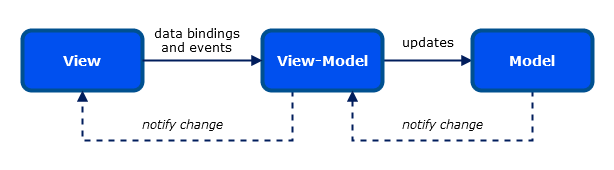
\includegraphics[width=0.8\textwidth]{images/mvvm.png}
   \caption{\gls{mvvm} design pattern overview, adapted from \parencite[7]{microsoft_mvvm}}
   \label{fig:mvvm}
 \end{figure}

\subsection{View}
The view is what the user sees. It is responsible for the structure, layout and appearance of the application.
\subsection{View-Model}
The view model implements event handlers and properties, to which the view can bind to. It also notifies the view of any changes to the underlying data. It defines the functionality, offered by the \gls{ui}, but the view determines how it is presented. 
\subsection{Model}
The model encapsulates the data of the application and validation of its logic.


\section{Vue.js}

Vue.js \parencite{vuejs_gh} is a progressive front end framework for building user interfaces and single-page applications based on the \gls{mvvm} design pattern described in \ref{sec:mvvm} \parencite{vuejs_book} \parencite{vuejs_guide}.  

\subsection{Components}
At the core of Vue.js are components, which are small, self-contained, composable and often reusable custom elements. Almost any type of application can be represented as a tree of components \parencite{vuejs_guide}. 

In more concrete terms, a Vue.js component is a single file with the extension of \code{.vue}, which consists of a \code{<template>}, \code{<script>} and optional \code{<style>}. The \code{template} is a HTML-based template, which can be parsed by specification compliant browsers and HTML parsers. It can contain other components or HTML elements and is equivalent to the \textit{view} in \gls{mvvm}. 

The \code{script} section of a Vue.js component includes the view-model of the component. Each component has a special JSON object \code{data}, equivalent to the \gls{mvvm} model.
The \code{script} part of a computed includes CSS-like styles.

\subsection{Data Binding}

Vue.js has built in support for \gls{databinding} using special directives.

\subsubsection{One-way Binding}
One-way binding is a one directional binding from source - a property of the model or other components to target - a property of a component or HTML tag. It can be achieved via the \code{v-bind} or \textit{moustache} syntax (double curly brackets). One-way bindings can also contain complex expressions.

\subsubsection{Two-way Binding}
Two-way binding is similar to one way-binding, but the value, which is bound to goes both ways and is synchronization. A typical example is a binding from an input field to a property of the model, e.g \code{email}. It can be achieved via the \code{v-model} binding directive.

\subsubsection{Event binding}
Event bindings are bindings of methods of the view model to events of components or HTML tags, for example the click of a button. It is done via the \code{v-on} or \code{@} directive. Event bindings can also contain anonymous methods.

\subsubsection{Computed Properties}
Computed properties are special properties, which can be used in \gls{databinding} and are a composition of other properties.

\subsubsection{V-for Binding}
A \code{v-for} directive is a special type of binding used to render lists, which semantically is used similarly to a \code{foreach} loop.

\section{ESLint}

ESLint \parencite{eslintMainPage} is a linting tool (linter) for ECMAScript/JavaScript. Linters are static code analysis tool, which are  used to flag and potentially automatically fix common code issues and enforce consistent code styling.

\subsection{Rules}
At the core of ESLint are rules, which are extensible pieces of code, bundled as plugins, that can be used to verify various aspects of code. An example would be a rule, which checks for matching closing parenthesis. 
Each rule consists of a \code{metadata} object
and a \code{create} function. The metadata object includes metadata such as documentation strings, the type of the rule and whether it is fixable or not. Based on type, rules can be either \textit{suggestions}, \textit{problems} or \textit{layout}. Suggestions indicate some improvement, but are not required and would not cause the linting to fail. Problems on the other hand would result in a linting failure. Layouts are rules that care mainly about the formatting of code, such as whitespaces, semicolons, etc. 

If the fixable property is specified, it indicates that the errors reported by this rule can be automatically fixed. This can be applied via the \code{--fix} command line option. It has two possible values - \textit{code} or \textit{whitespace} indicating the type of fixes, that this rule would apply. For example in \glspl{ide} fixable \textit{code} errors would show a fix shortcut displayed next to them and \textit{whitespace} rules could be applied when saving the file.

The \code{create} function is the implementation of the rule and takes as arguments a \code{context} and returns an object of methods which are called by ESLint for each node based on the \gls{visitor} pattern while traversing the \gls{ast}. 

\subsection{Selectors}
ESLint provides a very powerful matching mechanism for specifying what nodes to visit called selectors \parencite{eslintSelectors}. It is inspired by \textcite{estoolsEsQuery}.

Some notable selectors include:
\begin{itemize}
  \item AST Nodes \code{MemberExpression} - matches any node of type \code{MemberExpression}
  \item descendant \code{MemberExpression Identifier} - matches any node of type \code{Identifier} who has a descendant of type \code{MemberExpression} in the tree
  \item child \code{MemberExpression > Identifier}  - matches any node of type \code{Identifier} who has a direct parent (is a child of) of type \code{MemberExpression}
  \item :not \code{:not(MemberExpression)} - negation of a selector. In this case, matches any node, that is not a \code{MemberExpression} node.
  \item :matches - \code{:matches(MemberExpression, Identifier)} matches any of the selectors. In this case, either a \code{MemberExpression} or \code{Identifier}.
  \item attributes \code{Property[name=a]}. - Matches any AST Node, whose specified attribute has the specified value.
\end{itemize}

\subsection{AST Explorer}
An incredibly useful tool when working with \glspl{ast} is \gls{ast} Explorer, developed by \textcite{astexplorer_fkling2021Jan}. It enables the exploration of syntax trees generated by various parsers and also includes the vue-eslint-parser \parencite{eslint_vue_parser}.

\subsection{ESTree AST}
By default ESLint uses the Espree \parencite{eslintEspree} parser to parse JavaScript source code into an \gls{ast} defined in the ESTree specification \parencite{estreeASTSpec}. When Parsing \code{.vue} files ESLint uses this parser for the code inside the \code{<script>} tag.
  
\subsection{ESLint Parser Vue AST}

In order to parse the \code{<template>} section of \code{.vue} files, ESLint uses the vue-eslint-parser \parencite{eslint_vue_parser}. This parser outputs an  \gls{ast} compliant with their own \gls{ast} specification, defined in \parencite{eslint_vue_parser_ast}.